\documentclass[
    parskip=half,
    bibliography=totoc,     % Literatur im Inhaltsverzeichnis
    captions=tableheading,  % Tabellen�berschriften
    titlepage=firstiscover, % Titelseite ist Deckblatt
    ]{scrartcl}
    
\usepackage[top=2cm, bottom=4cm, left=2cm, right=2cm]{geometry}
\usepackage{color}
\usepackage[usenames,dvipsnames]{xcolor}
\definecolor{light-red}{HTML}{FFBABA}

% LaTeX2e korrigieren.
\usepackage{fixltx2e}

% Warnung, falls nochmal kompiliert werden muss
\usepackage[aux]{rerunfilecheck}

% Deutsche Spracheinstellungen
\usepackage{polyglossia}
\setmainlanguage{german}

% Unverzichtbare Mathe-Befehle
\usepackage{amsmath}

% Viele Mathe-Symbole
\usepackage{amssymb}

% Erweiterungen f�r amsmath
\usepackage{mathtools}

% Fonteinstellungen
\usepackage{fontspec}
\defaultfontfeatures{Ligatures=TeX}

\usepackage[
    math-style=ISO,    % \
    bold-style=ISO,    % |
    sans-style=italic, % | ISO-Standard folgen
    nabla=upright,     % |
    partial=upright,   % /
    ]{unicode-math}

\setmathfont{Latin Modern Math}
\setmathfont[range={\mathscr, \mathbfscr}]{XITS Math}
\setmathfont[range=\coloneq]{XITS Math}
\setmathfont[range=\propto]{XITS Math}

% Das hquer-Symbol versch�nern
\let\hbar\relax
\DeclareMathSymbol{\hbar}{\mathord}{AMSb}{"7E}
\DeclareMathSymbol{?}{\mathord}{AMSb}{"7E}

% Richtige Anf�hrungszeichen
\usepackage[autostyle]{csquotes}

% Zahlen und Einheiten
\usepackage[
  locale=DE,                   % Deutsche Einstellungen
  separate-uncertainty=true,   % Immer Fehler mit \pm
  per-mode=symbol-or-fraction, % m/s im Text, sonst Br�che
]{siunitx}

% Chemische Formeln
\usepackage[version=3]{mhchem}

% Sch�ne Br�che im Text
\usepackage{xfrac}

% Floats innerhalb einer Section halten
\usepackage[section, below]{placeins}

% Captions sch�ner machen.
\usepackage[
    labelfont=bf,        % Tabelle x: Abbildung y: ist jetzt fett
    font=small,          % Schrift etwas kleiner als Dokument
    width=0.9\textwidth, % Maximale Breite einer Caption schmaler
    ]{caption}

% Subfigure, subtable, subref
\usepackage{subcaption}

% Grafiken einbinden
\usepackage{graphicx}

% Gr��ere Variation von Dateinamen m�glich
\usepackage{grffile}

% Standardplatzierung f�r Floats einstellen
\usepackage{float}
\floatplacement{figure}{htbp}
\floatplacement{table}{htbp}

% Sch�ne Tabellen
\usepackage{booktabs}

% Seite drehen f�r breite Tabellen
\usepackage{pdflscape}

% Literaturverzeichnis
\usepackage{biblatex}

% Quellendatenbank
\addbibresource{lit.bib}
\addbibresource{programme.bib}

% Hyperlinks im Dokument
\usepackage[
    unicode,
    pdfusetitle,    % Titel, Autoren und Datum als PDF-Attribute
    pdfcreator={},  % PDF-Attribute s�ubern
    pdfproducer={}, % "
    ]{hyperref}
    
% Erweiterte Bookmarks im PDF
\usepackage{bookmark}

% Trennung von W�rtern mit Strichen
\usepackage[shortcuts]{extdash}

% Blindtext erzeugen
\usepackage{blindtext}

% Support f�r mdframed
\usepackage{kvoptions}
\usepackage{xparse}
\usepackage{etoolbox}
\usepackage{tikz}

% Sch�ne mehrseitige Rahmen um Text erzeugen
\usepackage{mdframed}
\mdfsetup{skipabove=\topskip,skipbelow=\topskip}
% Neue Mathematikbefehle
\DeclareMathOperator{\rank}{rang}
\DeclareMathOperator{\cond}{cond}
\newcommand{\up}{\mathup}
\newcommand{\R}{\mathbb{R}}
\newcommand{\N}{\mathbb{N}}
\newcommand{\upD}{\mathup{\Delta}}

% Wichtiger Befehl zur Erstellung einer blauen Box um einen Text
\newcommand\mybox[2][]{\tikz[overlay]\node[fill=blue!20,inner sep=4pt, anchor=text, rectangle, rounded corners=1mm,#1] {#2};\phantom{#2}}
\newenvironment{Versuch}[1]{
    \mdfsetup{
        innertopmargin=8pt,
        linecolor=blue!20,
        linewidth=2pt,
        topline=true,
        backgroundcolor=blue!20
        }
    \begin{mdframed}
    \Large{\textbf{#1}}
    \end{mdframed}}
    {}

\newenvironment{Stichworte}{
    \mdfsetup{
        frametitle={\mybox[fill=blue!20]{\Large{Stichworte}}},
        frametitleaboveskip=0pt,
        innertopmargin=10pt,
        linecolor=blue!20,
        linewidth=2pt,
        topline=true,
        backgroundcolor=white
        }
    \begin{mdframed}}
    {\end{mdframed}}    
    
\newenvironment{Zielsetzung}{
    \mdfsetup{
        frametitle={\mybox[fill=blue!20]{\Large{Zielsetzung}}},
        frametitleaboveskip=0pt,
        innertopmargin=10pt,
        linecolor=blue!20,
        linewidth=2pt,
        topline=true,
        backgroundcolor=white
        }
    \begin{mdframed}}
    {\end{mdframed}}

\newenvironment{Theorie}{
    \mdfsetup{
        frametitle={\mybox[fill=blue!20]{\Large{Theorie}}},
        frametitleaboveskip=0pt,
        innertopmargin=10pt,
        linecolor=blue!20,
        linewidth=2pt,
        topline=true,
        backgroundcolor=white
        }
    \begin{mdframed}}
    {\end{mdframed}}

\newenvironment{Durchführung}{
    \mdfsetup{
        frametitle={\mybox[fill=blue!20]{\Large{Durchführung}}},
        frametitleaboveskip=0pt,
        innertopmargin=10pt,
        linecolor=blue!20,
        linewidth=2pt,
        topline=true,
        backgroundcolor=white
        }
    \begin{mdframed}}
    {\end{mdframed}}
    
\newenvironment{Auswertung}{
    \mdfsetup{
        frametitle={\mybox[fill=blue!20]{\Large{Auswertung}}},
        frametitleaboveskip=0pt,
        innertopmargin=10pt,
        linecolor=blue!20,
        linewidth=2pt,
        topline=true,
        backgroundcolor=white
        }
    \begin{mdframed}}
    {\end{mdframed}}
    
\newenvironment{Diskussion}{
    \mdfsetup{
        frametitle={\mybox[fill=blue!20]{\Large{Diskussion}}},
        frametitleaboveskip=0pt,
        innertopmargin=10pt,
        linecolor=blue!20,
        linewidth=2pt,
        topline=true,
        backgroundcolor=white
        }
    \begin{mdframed}}
    {\end{mdframed}}

\newenvironment{Merke}{
    \mdfsetup{
        frametitle={\mybox[fill=red]{\Large{Merke}}},
        frametitleaboveskip=0pt,
        innertopmargin=5pt,
        linecolor=red,
        linewidth=1pt,
        topline=true,
        backgroundcolor=light-red
        }
    \begin{mdframed}}
    {\end{mdframed}}

\newenvironment{Appendix}{
    \mdfsetup{
        frametitle={\mybox[fill=blue!20]{\Large{Appendix}}},
        frametitleaboveskip=0pt,
        innertopmargin=10pt,
        linecolor=blue!20,
        linewidth=0pt,
        topline=false,
        backgroundcolor=white
        }
    \begin{mdframed}}
    {\end{mdframed}}
    
\begin{document}

    \begin{Versuch}{V303: Lock In-Verstärker}
	\begin{Stichworte}
		Verstärker in der Messtechnik,
		Filter aus Spulen und Kondensatoren	
	\end{Stichworte}

	\begin{Zielsetzung}
		Die Funktionsweise des Lock In-Verstärkers - ein wichtiges Messinstrument von vergleichbarer Wichtigkeit wie ein Oszilloskop - verstehen und erklären.
	\end{Zielsetzung}

    \begin{Theorie}
    	Der Lock In-Verstärker ist ein Messinstrument, mit welchem schwache Signale einerseits verstärkt und andererseits vom  Rauschen befreit werden kann.
    	Vor allem schwache Signale neigen dazu, von Rauschen überdeckt zu werden, schlichtes Verstärken von schwachen Signalen wird durch auftretendes starkes Rauschen unbrauchbar.
    	Ist die Frequenz eines Signales bekannt, beispielsweise AM-Radio einer bekannten Frequenz, so ist es möglich, 
    	Rauschen zu eliminieren.
    	Die Ausgabe des Lock In-Verstärkers ist eine Gleichspannung als Maß für die Amplitude der eingestellten Frequenz.

    	Die Funktionsweise ist anhand dieses schematischen Aufbaus gut erklärbar. 
    	\centering
    	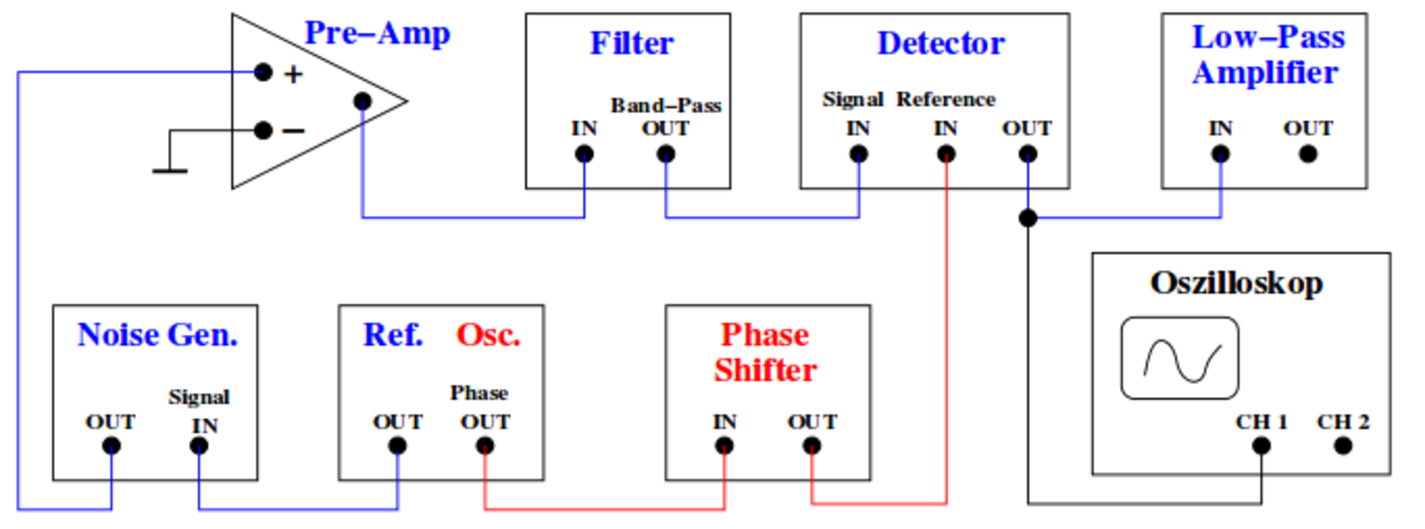
\includegraphics[width=0.9\textwidth]{build/Bilder/LockIn.pdf}
    	\flushleft
    	Nach der Verstärkung durch den \emph{Pre-Amplifier} durchläuft das Signal zunächst einen \emph{Bandpassfilter}:
		alle Frequenzen $\omega<<\omega_0$ und $\omega>>\omega_0$ werden grob herausgefiltert, das Frequenz-Rauschen wird minimiert. 
		Ein \emph{Funktionsgenerator} erzeugt die Referenzspannung $U_\mathup{ref}$ -- eine Sinus- oder Rechteckspannung der Frequenz $\omega_0$ -- , welche über den \emph{Phasenschieber} an die Phase des Eingangssignals angepasst werden kann. 
		Dieser Vorgang nennt sich Synchronisation.
		Im \emph{Mischer} treffen beide Signale aufeinander und werden per Signalfaltung multipliziert. 
		Anschließend wird das Mischsignal $U_\mathup{sig}\times U_\mathup{ref}$ an den \emph{Tiefpass} weitergeleitet, der die Modulationsfrequenz $\omega_0$ über mehrere Perioden integriert, um restliche Rauschanteile $\omega\neq\omega_0$ auszuschließen. 
		Dieser Tiefpass hat die Funktion eines dämpfenden Gleichrichters: schnelle Amplitudenänderung, also Amplitudenrauschen, werden durch die Integration herausgedämpft.
		Zurück bleiben nur die Anteile der Signalsspannung $U_\mathup{sig}$, die mit der Referenzspannung synchronisiert werden konnten.
		Um eine möglichst geringe Bandbreite $\upD{\nu}=\frac{1}{\pi RC}$ zu erhalten, sollte die Zeitkonstante $\uptau=RC$ des \emph{Tiefpasses} ausreichend groß gewählt werden. 
		Damit wird eine hohe Güteziffer im Bezug auf Störungsfilterung erzielt.

		\centering
    	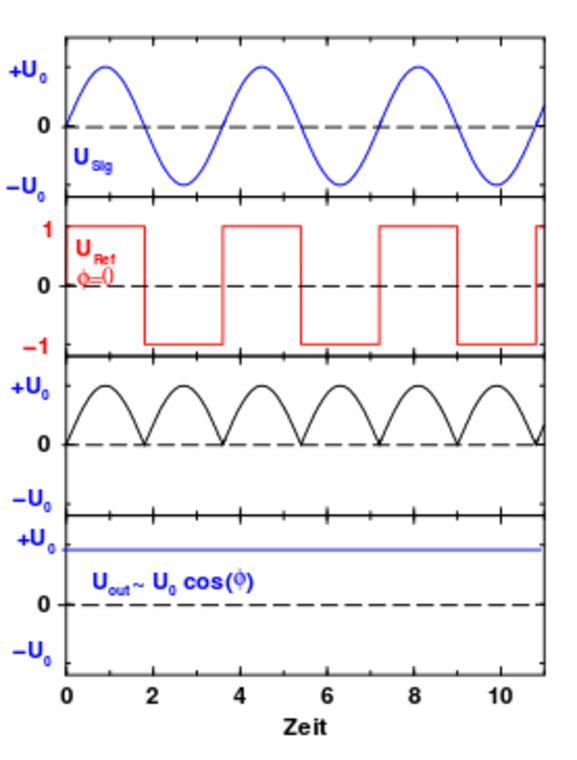
\includegraphics[width=0.4\textwidth]{build/Bilder/Signal.pdf}
    	\flushleft

    	Wird beispielsweise ein Sinus-förmiges Eingangssignal $U_\mathup{sig}=U_0 \sin(\omega t)$ mit einem rechteckigen normierten Referenzsignal $U_\mathup{ref}$ gleicher Frequenz gefaltet, wird diese zunächst durch eine Fourierreihe angenähert, welche aus den ungeraden Harmonischen der Grundfrequenz besteht. 
		Wird das multiplizierte Signal,  bestehend aus geraden Oberwellen der Frequenz $\omega$, durch den Tiefpass geleitet, ergibt sich die Endspannung
		\begin{equation}
			U_\mathup{out}=\frac{2}{\pi}U_0\text{cos}(\upD\Phi).
			\label{cos}
		\end{equation}
		Besteht kein Phasenunterschied zwischen Eingangs- und Referenzsignal, so nimmt die Endspannung ihren Maximalwert an.

		Gewissermaßen zeigt ein Lock In-Verstärker über seine DC-Spannungsausgabe, wie groß die Amplitude der eingestellten Frequenz im Eingangssignal ist.

	\end{Theorie}
    
    \begin{Durchführung}
    	Die Funktionsweise des Verstärkers, den einzelnen Komponenten nach, mit einem Oszilloskop sichtbar machen.
    	Hierzu wird einerseits ein ungestörtes Signal und das gleiche Signal mit Störung und andererseits ein LED-Signal verwendet.
    	Beim gestörten Signal wird die Phasenverschiebung benützt, um die Gleichung \eqref{cos} zu bestätigen. Die Messung eines gepulsten LED-Signals geschieht ohne Abdeckung oder andere optische Bemühung.

    	Die Oszilloskopenbilder von dem Rohsignal, dem gefalteten Signal und der Ausgabe am Ende werden aufgenommen.
    \end{Durchführung}        
    
    \begin{Auswertung}
    	Durchgehen gute Ergebnisse:
    	\begin{itemize}
    		\item Differenz der Ausgangsspannung bei ungestörtem Signal und bei gleichem Signal mit Störung ist gering.
    		\item Der Cosinus-Zusammenhang zwischen Endspannung und Phasenverschiebung konnte gut nachgewiesen werden.
    		\item Das LED-Signal konnte über einen Meter Distanz überwinden und trotzdem verlässlich gemessen werden.
    	\end{itemize}
    \end{Auswertung}

    \begin{Diskussion}
 		Der Lock In-Verstärker eignet sich hervorragend zur Messung von schwachen und gestörten Signalen. 
 		Das Signal kann dabei Störungen aufweisen, die die Signalstärke wesentlich übertreffen.
 		Im Versuch wurde die Störsicherheit bei üblichem Verhältnis von Störung zu Signal nachgewiesen.
    \end{Diskussion}

    \begin{Merke}
    	Lock In-Verstärker sind toll.
		Geeignet für Übermittlung von Daten über langen Strecken.

		Unterschied zum Band-Pass: der Lock In-Filter ist in der Lage, Signale mit variabler Frequenz zu verstärken und Störung in Frequenzlage zu filtern.
    \end{Merke}

    \end{Versuch}
\end{document}